\chapter{Případy užití a požadavky na aplikaci}

Tato kapitola se zabývá specifikací požadavků na navrhovanou aplikaci a případy užití, které tyto požadavky ilustrují. Nejprve jsou definovány pojmy a terminologie (viz tabulka č. \ref{tab:definice-pojmu}) používané v kontextu požadavků a případů užití, aby bylo zajištěno jednoté porozumění mezi všemi zainteresovanými stranami. Následuje sekce č. \ref{kap:usecase} zabývající se případy užití  a jejich aktéry. Předposlední sekce č. \ref{sekce:funkcni-pozadavky} a poslední sekce č. \ref{sekce:nefunkcni-pozadavky} jsou věnovány systémovým požadavkům, které jsou s případy užití úzce spjaty.

Pro tuto kapitolu byla převzata struktura ze šablon metodiky MMSP\footnote{https://spicenter.vse.cz/wp-content/uploads/metodiky/publikovana\_MMSP/index.htm}, která je určena pro malé týmy a využívá metodiky FURPS+ pro stanovování požadavků \parencite{rejnkovaLokalizacePrizpusobeniMetodiky}. Nutno podotknout, že šablony nebyly použity v zcela identické podobě. Napříč šablonami byla vynechána verzovací část, která z hlediska rozsahu práce není relevantní a šablony byly přeneseny z dokumentu ve formátu MS Word (.docx) do \LaTeX u, což vedlo k úpravě formátování a struktury některých částí. Nicméně, základní logika a obsah šablon zůstaly zachovány.

\begin{longtable}{L{3.5cm} L{11cm}}
  \caption{Slovník pojmů}\label{tab:definice-pojmu}\\
  \toprule
  \textbf{Pojem} & \textbf{Definice} \\
  \midrule
  \endfirsthead
  \multicolumn{2}{l}{\textit{Pokračování tabulky \ref{tab:definice-pojmu}}} \\
  \toprule
  \textbf{Pojem} & \textbf{Definice} \\
  \midrule
  \endhead
  \midrule
  \multicolumn{2}{r}{\textit{Pokračování na další stránce}} \\
  \endfoot
  \bottomrule
  \endlastfoot
    musí & Vyjadřuje závaznost něčeho. \\
    nesmí & Vyjadřuje naprostý zákaz něčeho. \\
    může & Vyjadřuje volitelnost něčeho. \\
    smí & Vyjadřuje oprávnění k~něčemu. \\
    má / měl by / doporučuje se & Vyjadřuje slabší závaznost. \\
    IEQ & Zkratka anglického \emph{Indoor Environmental Quality}, tedy kvalita vnitřního prostředí. Jde o~zastřešující pojem pokrývající čtyři kategorie, a~to kvalitu vnitřního ovzduší, tepelný komfort, vizuální komfort a~akustický komfort. \\
    IAQ & Zkratka anglického \emph{Indoor Air Quality}, tedy kvalita vnitřního ovzduší. Jedná se o~podmnožinu IEQ zaměřenou na koncentrace plynů a~aerosolů (CO\textsubscript{2}, mikročástice, těkavé organické látky aj.). \\
    VZT & Vzduchotechnika, tedy soustava zařízení zajišťující řízenou výměnu vzduchu v~budově (přívod, odvod, filtraci, případně úpravu teploty a~vlhkosti). \\
    rekuperace & Zpětné získávání tepla z~odváděného vzduchu. Výměník v~jednotce VZT předává teplo (případně vlhkost) z~odpadního vzduchu do vzduchu přiváděného do budovy, čímž snižuje energetické nároky na vytápění. \\
    dlouhodobý / krátkodobý / průchozí pobyt & Kategorizace místnosti podle typické doby, kterou v~ní osoby tráví. \emph{Dlouhodobý} odpovídá pobytovým místnostem (ložnice, kancelář, učebna), \emph{krátkodobý} prostorům s~opakovanou kratší přítomností (kuchyně, koupelna, jednací místnost) a~\emph{průchozí} místům občasného nebo přechodného užívání (chodba, schodiště, sklad). \\
    dýchací zóna & Výškové pásmo nad podlahou, ve kterém se obvykle nachází hlava člověka při běžných činnostech a~v~němž je proto měření kvality vnitřního prostředí nejreprezentativnější vůči expozici osob. \\
    entita & Samostatná, jednoznačně rozlišitelná věc reálného nebo informačního světa, kterou systém eviduje (typicky budova, místnost, senzor, pozorování). Každá entita má jednoznačnou identitu a~sadu atributů, prostřednictvím nichž je v~systému popsána. \\
    subjekt zájmu & Entita reálného světa, jejíž vlastnost je předmětem měření, v~kontextu této práce typicky místnost. Odpovídá třídě \texttt{sosa:FeatureOfInterest} ontologie SSN/SOSA. \\
    veličina & Pozorovatelná vlastnost subjektu zájmu, kterou senzor měří (např. teplota, koncentrace CO\textsubscript{2}, hladina akustického tlaku). Odpovídá třídám \texttt{sosa:ObservableProperty} v~SSN/SOSA a~\texttt{qudt:QuantityKind} ve slovníku QUDT. \\
    jednotka & Standardizovaná měrná škála, v~níž je vyjádřena hodnota veličiny (např. $^{\circ}$C, ppm, $\mu$g/m\textsuperscript{3}). Odpovídá třídě \texttt{qudt:Unit} ve slovníku QUDT, který umožňuje strojový převod mezi ekvivalentními jednotkami. \\
    pozorování & Akt pořízení jedné hodnoty určité veličiny senzorem v~daném okamžiku na konkrétním subjektu zájmu, v~práci synonymum pro \emph{měření}. Odpovídá třídě \texttt{sosa:Observation} ontologie SSN/SOSA. \\
    SSN/SOSA & Doporučení W3C definující dvojici provázaných ontologií pro popis senzorů a~pozorování. \emph{SOSA} (Sensor, Observation, Sample, Actuator) je odlehčené jádro, \emph{SSN} (Semantic Sensor Network) přidává systémovou nadstavbu pro kompozici a~kapacity zařízení. \\
    QUDT & Otevřený slovník publikovaný organizací QUDT.org popisující veličiny (\emph{Quantities}), jednotky (\emph{Units}), dimenze (\emph{Dimensions}) a~datové typy (\emph{Types}). Poskytuje URI identifikátory veličin a~jednotek a~koeficienty pro strojový převod mezi nimi. \\
    OFN & Otevřené formální normy publikované Digitální a~informační agenturou (DIA) podle zákona č.\,106/1999\,Sb. Stanovují technické požadavky na publikaci otevřených dat orgány veřejné správy, mimo jiné na strukturu, formát, kódování, schéma a~katalogizační metadata. \\
    DCAT-AP-CZ & Česká aplikační profilace evropského standardu DCAT-AP pro popis datových katalogů. Definuje strojově čitelná katalogizační metadata otevřených datových sad (název, popis, vydavatel, licence, klíčová slova, distribuce) ve formátu RDF. \\
    přihlášená relace & Stav navázaný úspěšným přihlášením uživatele, ve kterém systém přiřazuje příchozí požadavky konkrétnímu autentizovanému uživateli a zpřístupňuje mu funkce vyžadující autentizaci. Trvá do explicitního odhlášení, vypršení časového limitu nebo invalidace ze strany systému. \\
\end{longtable}

\section{Případy užití}

Pro ilustrování funkcionality navrhovaného systému a jeho iterakcí s entitami vnějšího světa byly stanoveny případy užití (viz tabulky č. \ref{tab:usecase:UC01}, \ref{tab:usecase:UC02}, \ref{tab:usecase:UC03}, \ref{tab:usecase:UC04}, \ref{tab:usecase:UC05}, \ref{tab:usecase:UC06}, \ref{tab:usecase:UC07}, \ref{tab:usecase:UC08}, \ref{tab:usecase:UC09}, \ref{tab:usecase:UC10}, \ref{tab:usecase:UC11}, \ref{tab:usecase:UC12}, \ref{tab:usecase:UC13}, \ref{tab:usecase:UC14}, \ref{tab:usecase:UC15}, \ref{tab:usecase:UC16}, \ref{tab:usecase:UC17}). Tyto případy užití jsou vizualizovány pomocí diagramu UML případů užití na obrázku č. \ref{obr:usecase}.

\begin{figure}[p]
    \centering
    \resizebox{0.96\textwidth}{!}{%
    \begin{tikzpicture}[
      uc/.style={ellipse, draw, align=center, minimum width=2.8cm, minimum height=1.0cm,
                 font=\scriptsize, inner sep=2pt},
      assoc/.style={draw},
      incl/.style={draw, dashed, -latex, font=\scriptsize},
    ]

    %--- HRANICE SYSTÉMŮ ---%

    % Hlavní systémová hranice
    \draw[thick] (2.2, -0.5) rectangle (14.5, 15.5);
    \node[anchor=north west, font=\normalsize\bfseries] at (2.2, 15.5)
      {Aplikace pro sběr dat IEQ};

    % Autentizační subsystém
    \draw (7.0, 7.5) rectangle (14.2, 15.0);
    \node[anchor=north east, font=\small] at (14.2, 15.0)
      {Autentizační služba};

    %--- PŘÍPADY UŽITÍ: AUTENTIZACE ---%

    \node[uc] (uc-auth)    at (8.7,  12.5) {Autentizace};
    \node[uc] (uc-reg)     at (12.0, 14.0) {Registrace\\do systému};
    \node[uc] (uc-login)   at (12.3, 12.5) {Přihlášení\\do systému};
    \node[uc] (uc-logout)  at (12.0, 10.8) {Odhlášení\\ze systému};
    \node[uc] (uc-chgcred) at (11.8,  9.1) {Změna\\přihlašovacích\\údajů};

    %--- PŘÍPADY UŽITÍ: SPRÁVA PROSTOR A SENZORŮ ---%

    \node[uc] (uc-building) at (5.0, 13.5) {Evidence budovy};
    \node[uc] (uc-room)     at (5.0, 11.8) {Evidence místnosti};
    \node[uc] (uc-params)   at (5.0, 10.1) {Změna parametrů\\s čas. platností};
    \node[uc] (uc-sens-reg) at (5.0,  8.4) {Registrace senzoru};
    \node[uc] (uc-sens-lc)  at (5.0,  6.7) {Správa živ. cyklu\\senzoru};

    %--- PŘÍPADY UŽITÍ: POZOROVÁNÍ ---%

    \node[uc] (uc-obs)      at (7.3,  5.2) {Příjem a validace\\pozorování};

    %--- PŘÍPADY UŽITÍ: VEŘEJNÉ API ---%

    \node[uc] (uc-api)      at (8.8,  3.8) {Čtení dat\\přes veřejné API};
    \node[uc] (uc-filter)   at (10.0,  6.5) {Filtrování dotazů\\na čtecí API};
    \node[uc] (uc-page)     at (12.8, 4.8) {Procházení str.\\odpovědí API};
    \node[uc] (uc-search)   at (12.8, 3.0) {Vyhledání entit\\dle parametrů};
    \node[uc] (uc-schema)   at (10, 1.7) {Získání str. čit.\\popisu API};

    %--- PŘÍPADY UŽITÍ: DATA ---%

    \node[uc] (uc-harvest)  at (5.0, 2.5) {Harvestování\\str. čit. metadat};
    \node[uc] (uc-download) at (5.0, 0.9) {Stažení archivu\\naměřených dat};

    %--- AKTÉŘI ---%

    \ucactor{a-oper}      {0.7}{10.0}{Provozovatel\\monitorovaného\\prostoru}
    \ucactor{a-sensor}    {1.2}{ 7.5}{Senzor}
    \ucactor{a-dev}       {1.2}{ 5.5}{Vývojář aplikací\\třetí strany}
    \ucactor{a-catalog}   {1.2}{ 3.2}{Datový katalog}
    \ucactor{a-researcher}{1.2}{ 1.2}{Výzkumný\\pracovník}
    \ucactor[2.2cm]{a-email}{16.0}{12.5}{«Service»\\Emailová služba}

    %--- ASOCIACE: AKTÉR → PŘÍPAD UŽITÍ ---%

    \draw[assoc] (a-oper)       -- (uc-auth);
    \draw[assoc] (a-oper)       -- (uc-building);
    \draw[assoc] (a-oper)       -- (uc-room);
    \draw[assoc] (a-oper)       -- (uc-params);
    \draw[assoc] (a-oper)       -- (uc-sens-reg);
    \draw[assoc] (a-oper)       -- (uc-sens-lc);
    \draw[assoc] (a-sensor)     -- (uc-obs);
    \draw[assoc] (a-dev)        -- (uc-api);
    \draw[assoc] (a-catalog)    -- (uc-harvest);
    \draw[assoc] (a-researcher) -- (uc-download);

    %--- ASOCIACE: PŘÍPAD UŽITÍ → EMAILOVÁ SLUŽBA ---%

    \draw[assoc] (uc-reg)     -- (a-email);
    \draw[assoc] (uc-chgcred) -- (a-email);

    %--- RELACE «INCLUDE»: AUTENTIZACE ---%

    \draw[incl] (uc-reg)
      -- node[above, sloped, font=\tiny] {«include»} (uc-auth);
    \draw[incl] (uc-login)
      -- node[above, font=\tiny]         {«include»} (uc-auth);
    \draw[incl] (uc-logout)
      -- node[above, sloped, font=\tiny] {«include»} (uc-auth);
    \draw[incl] (uc-chgcred)
      -- node[above, sloped, font=\tiny] {«include»} (uc-auth);

    %--- RELACE «INCLUDE»: VEŘEJNÉ API ---%

    \draw[incl] (uc-filter)
      -- node[right, font=\tiny] {«include»} (uc-api);
    \draw[incl] (uc-page)
      -- node[above, sloped, font=\tiny] {«include»} (uc-api);
    \draw[incl] (uc-search)
      -- node[above, sloped, font=\tiny] {«include»} (uc-api);
    \draw[incl] (uc-schema)
      -- node[above, sloped, font=\tiny] {«include»} (uc-api);

    \end{tikzpicture}
    }
    \caption{Diagram případů užití}
    \label{obr:usecase}
\end{figure}

  \subsection{Definice aktérů}

  \begin{longtable}{L{4cm} p{10cm}}
    \caption{Definice aktérů}
    \label{tab:definice-akteru}\\
    \toprule
    \textbf{Název aktéra} & \textbf{Popis aktéra} \\
    \midrule
    \endfirsthead
    \multicolumn{2}{l}{\textit{Pokračování tabulky \ref{tab:definice-akteru}}} \\
    \toprule
    \textbf{Název aktéra} & \textbf{Popis aktéra} \\
    \midrule
    \endhead
    \midrule
    \multicolumn{2}{r}{\textit{Pokračování na další stránce}} \\
    \endfoot
    \bottomrule
    \endlastfoot
    Provozovatel monitorovaného prostoru & Subjekt odpovědný za prostor, ve kterém probíhá měření (instituce, firma, vlastník budovy, škola, úřad). Registruje se v systému, eviduje monitorované budovy, místnosti a senzory a prostřednictvím systému publikuje pořízená měření. \\
    Vývojář aplikací třetí strany & Vývojář integrující IEQ data do vlastních aplikací nebo systémů (mobilní aplikace, dashboardy, integrace se systémy řízení budov). Pracuje s daty strojově prostřednictvím veřejného čtecího API a očekává stabilní, zdokumentovaný a předvídatelný způsob přístupu k datům. \\
    Výzkumný pracovník & Akademik nebo analytik využívající otevřená IEQ data pro výzkum (například vliv prostředí na zdraví a produktivitu). Pracuje s historickými daty hromadně a napříč více měřicími body; pro tyto účely stahuje publikovaný archiv naměřených dat ve strojově čitelném otevřeném formátu. \\
    Senzor & Strojový aktér -- evidované měřicí zařízení odesílající systému pozorování (měření) určité veličiny u subjektu zájmu. Komunikuje výhradně strojově prostřednictvím rozhraní pro příjem měření, identifikuje se v systému evidovaným jednoznačným identifikátorem zařízení a řídí se deklarovanými veličinami a jednotkami ze slovníku QUDT. \\
    Datový katalog & Strojový aktér -- externí katalog otevřených dat (např. Národní katalog otevřených dat), který automatizovaně harvestuje katalogizační metadata o publikovaných datových sadách systému ve formátu odpovídajícím standardu DCAT-AP. Slouží k tomu, aby konzumenti dat mohli datovou sadu objevit a propojit s dalšími otevřenými daty. \\
    Návštěvník & Anonymní uživatel veřejného webového rozhraní aplikace, který si bez registrace prohlíží mapu subjektů zájmu a~jejich aktuální i~historická měření. S~daty pracuje vizuálně, prostřednictvím veřejně dostupného uživatelského rozhraní, jež samo vystupuje jako konzument veřejného čtecího API. \\
\end{longtable}


\subsection{Specifikace případů užití}


První případ užití je specifikován v tabulce č. \ref{tab:usecase:UC01}.

\begin{UseCaseTable}
  {Registrace do systému}
  {UC01}
  {F01}
  {Vytvoření účtu provozovatele monitorovaného prostoru za účelem evidence a publikace měření}
  {Provozovatel monitorovaného prostoru}
  {Emailová služba}
  {Uživatel není v systému evidován}
  {Uživatel je v systému evidován v neaktivním stavu, byl odeslán potvrzovací email s odkazem pro aktivaci účtu}

\UseCaseScenario{Základní scénář}
\UseCaseStep{uživatel}{Otevře domovskou stránku a klikne na tlačítko pro registraci.}
\UseCaseStep{systém}{Vrátí registrační formulář.}
\UseCaseStep{uživatel}{Vyplní email a heslo a formulář odešle.}
\UseCaseStep{systém}{Ověří, že zadaný email dosud není registrován.}
\UseCaseStep{systém}{Vytvoří uživatelský účet v neaktivním stavu.}
\UseCaseStep{systém}{Odešle na zadaný email zprávu s odkazem pro aktivaci účtu.}

\UseCaseScenario{Alternativní scénář -- email již registrován}
\UseCaseStepCustom{A1}{uživatel, systém}{shodné s kroky 1--3 základního scénáře.}
\UseCaseStepCustom{A2}{systém}{Zjistí, že zadaný email je již registrován, a vyzve uživatele k zadání jiného emailu.}
\UseCaseStepCustom{A3}{uživatel}{Zadá jiný email.}
\UseCaseStepCustom{A4}{systém}{Pokračuje krokem 4 základního scénáře.}

\end{UseCaseTable}



Druhý případ užití je specifikován v tabulce č. \ref{tab:usecase:UC02}.

\begin{UseCaseTable}
  {Přihlášení do systému}
  {UC02}
  {F02}
  {Zahájení přihlášené relace umožňující správu evidovaných subjektů zájmu}
  {Provozovatel monitorovaného prostoru}
  {}
  {Uživatel je v systému evidován v aktivním stavu, není přihlášen}
  {Uživatel je přihlášen}

\UseCaseScenario{Základní scénář}
\UseCaseStep{uživatel}{Otevře přihlašovací stránku.}
\UseCaseStep{systém}{Vrátí přihlašovací formulář.}
\UseCaseStep{uživatel}{Vyplní email a heslo použité při registraci a formulář odešle.}
\UseCaseStep{systém}{Ověří, že zadané údaje odpovídají evidovanému uživateli v aktivním stavu.}
\UseCaseStep{systém}{Zahájí přihlášenou relaci a přesměruje uživatele do administračního rozhraní.}

\UseCaseScenario{Alternativní scénář -- neplatné údaje}
\UseCaseStepCustom{A1}{uživatel, systém}{shodné s kroky 1--3 základního scénáře.}
\UseCaseStepCustom{A2}{systém}{Zjistí, že zadané údaje neodpovídají žádnému evidovanému uživateli, a vyzve uživatele k jejich opětovnému zadání.}
\UseCaseStepCustom{A3}{uživatel}{Zadá údaje znovu.}
\UseCaseStepCustom{A4}{systém}{Pokračuje krokem 4 základního scénáře.}

\UseCaseScenario{Alternativní scénář -- neaktivní účet}
\UseCaseStepCustom{B1}{uživatel, systém}{shodné s kroky 1--3 základního scénáře.}
\UseCaseStepCustom{B2}{systém}{Zjistí, že účet je evidován v neaktivním stavu, a vyzve uživatele k aktivaci účtu přes odkaz v potvrzovacím emailu.}

\end{UseCaseTable}



Třetí případ užití je specifikován v tabulce č. \ref{tab:usecase:UC03}.

\begin{UseCaseTable}
  {Odhlášení ze systému}
  {UC03}
  {F03}
  {Ukončení přihlášené relace přihlášeného uživatele}
  {Provozovatel monitorovaného prostoru}
  {}
  {Uživatel je přihlášen}
  {Uživatel není přihlášen, přihlášená relace byla ukončena}

\UseCaseScenario{Základní scénář}
\UseCaseStep{uživatel}{V administraci klikne na tlačítko pro odhlášení.}
\UseCaseStep{systém}{Ukončí přihlášenou relaci a invaliduje její identifikátor.}
\UseCaseStep{systém}{Přesměruje uživatele na domovskou stránku.}

\end{UseCaseTable}



Čtvrtý případ užití je specifikován v tabulce č. \ref{tab:usecase:UC04}.

\begin{UseCaseTable}
  {Změna přihlašovacích údajů}
  {UC04}
  {F04}
  {Aktualizace emailu nebo hesla přihlášeného uživatele}
  {Provozovatel monitorovaného prostoru}
  {}
  {Uživatel je přihlášen}
  {Přihlašovací údaje uživatele jsou aktualizovány}

\UseCaseScenario{Základní scénář}
\UseCaseStep{uživatel}{V administraci otevře nastavení účtu.}
\UseCaseStep{systém}{Vrátí formulář pro změnu emailu a hesla.}
\UseCaseStep{uživatel}{Vyplní nový email či heslo, zadá pro potvrzení stávající heslo a formulář odešle.}
\UseCaseStep{systém}{Ověří, že stávající heslo odpovídá uloženému heslu uživatele.}
\UseCaseStep{systém}{Aktualizuje přihlašovací údaje uživatele a zobrazí potvrzení.}

\UseCaseScenario{Alternativní scénář -- neplatné stávající heslo}
\UseCaseStepCustom{A1}{uživatel, systém}{shodné s kroky 1--3 základního scénáře.}
\UseCaseStepCustom{A2}{systém}{Zjistí, že zadané stávající heslo neodpovídá uloženému, a vyzve uživatele k jeho opětovnému zadání.}
\UseCaseStepCustom{A3}{uživatel}{Zadá stávající heslo znovu.}
\UseCaseStepCustom{A4}{systém}{Pokračuje krokem 4 základního scénáře.}

\UseCaseScenario{Alternativní scénář -- email je již používán}
\UseCaseStepCustom{B1}{uživatel, systém}{shodné s kroky 1--4 základního scénáře.}
\UseCaseStepCustom{B2}{systém}{Zjistí, že nový email je již používán jiným účtem, a vyzve uživatele k zadání jiného.}
\UseCaseStepCustom{B3}{uživatel}{Zadá jiný email.}
\UseCaseStepCustom{B4}{systém}{Pokračuje krokem 5 základního scénáře.}

\end{UseCaseTable}



Pátý případ užití je specifikován v tabulce č. \ref{tab:usecase:UC05}.

\begin{UseCaseTable}
  {Evidence budovy}
  {UC05}
  {F05}
  {Zaregistrování budovy do evidence systému}
  {Provozovatel monitorovaného prostoru}
  {}
  {Uživatel je přihlášen}
  {Budova je v systému evidována}

\UseCaseScenario{Základní scénář}
\UseCaseStep{uživatel}{V administraci zvolí akci pro založení budovy.}
\UseCaseStep{systém}{Vrátí formulář pro evidenci budovy se základními a doplňujícími údaji.}
\UseCaseStep{uživatel}{Vyplní povinné základní údaje (název, adresa, typ), volitelně doplňující údaje (souřadnice, rok výstavby, rok poslední rekonstrukce, úroveň veřejného zobrazení polohy) a formulář odešle.}
\UseCaseStep{systém}{Ověří, že povinné údaje jsou vyplněny a všechny zadané údaje jsou v platném tvaru.}
\UseCaseStep{systém}{Uloží budovu do evidence a zobrazí potvrzení.}

\UseCaseScenario{Alternativní scénář -- neplatné údaje}
\UseCaseStepCustom{A1}{uživatel, systém}{shodné s kroky 1--3 základního scénáře.}
\UseCaseStepCustom{A2}{systém}{Zjistí chybu ve vyplnění formuláře (chybí povinné pole, neplatný formát hodnoty) a vyzve uživatele k její opravě.}
\UseCaseStepCustom{A3}{uživatel}{Opraví zadané údaje.}
\UseCaseStepCustom{A4}{systém}{Pokračuje krokem 4 základního scénáře.}

\end{UseCaseTable}



Šestý případ užití je specifikován v tabulce č. \ref{tab:usecase:UC06}.

\begin{UseCaseTable}
  {Evidence místnosti}
  {UC06}
  {F06}
  {Zaregistrování místnosti u evidované budovy}
  {Provozovatel monitorovaného prostoru}
  {}
  {Uživatel je přihlášen, evidovaná budova existuje}
  {Místnost je v systému evidována pod konkrétní budovou}

\UseCaseScenario{Základní scénář}
\UseCaseStep{uživatel}{V detailu evidované budovy zvolí akci pro založení místnosti.}
\UseCaseStep{systém}{Vrátí formulář pro evidenci místnosti se základními a doplňujícími údaji.}
\UseCaseStep{uživatel}{Vyplní povinné základní údaje (název, podlaží), volitelně doplňující údaje (funkce místnosti z předdefinovaného číselníku, typická délka pobytu, kategorie zdrojů znečištění, podlahová plocha, světlá výška, způsob větrání) a formulář odešle.}
\UseCaseStep{systém}{Ověří, že povinné údaje jsou vyplněny, všechny zadané údaje jsou v platném tvaru a hodnoty z číselníků odpovídají povoleným položkám.}
\UseCaseStep{systém}{Uloží místnost do evidence pod zvolenou budovou a zobrazí potvrzení.}

\UseCaseScenario{Alternativní scénář -- neplatné údaje}
\UseCaseStepCustom{A1}{uživatel, systém}{shodné s kroky 1--3 základního scénáře.}
\UseCaseStepCustom{A2}{systém}{Zjistí chybu ve vyplnění formuláře (chybí povinné pole, neplatný formát hodnoty, neznámá položka číselníku) a vyzve uživatele k její opravě.}
\UseCaseStepCustom{A3}{uživatel}{Opraví zadané údaje.}
\UseCaseStepCustom{A4}{systém}{Pokračuje krokem 4 základního scénáře.}

\end{UseCaseTable}



Sedmý případ užití je specifikován v tabulce č. \ref{tab:usecase:UC07}.

\begin{UseCaseTable}
  {Změna parametrů s časovou platností}
  {UC07}
  {F07}
  {Aktualizace parametrů subjektu zájmu nebo senzoru s platností od zadaného data při zachování návaznosti starších měření na původní parametry}
  {Provozovatel monitorovaného prostoru}
  {}
  {Uživatel je přihlášen, subjekt zájmu (budova, místnost) nebo senzor je v systému evidován}
  {V evidenci je uložena nová verze parametrů s platností od zadaného data, předchozí verze parametrů zůstává platná pro období do tohoto data, historická měření zůstávají vázána na verzi parametrů platnou v době jejich pořízení}

\UseCaseScenario{Základní scénář}
\UseCaseStep{uživatel}{V detailu evidovaného subjektu zájmu nebo senzoru zvolí akci pro úpravu parametrů.}
\UseCaseStep{systém}{Vrátí formulář s aktuálně platnými parametry a polem pro datum, od kdy mají nové hodnoty platit.}
\UseCaseStep{uživatel}{Upraví hodnoty parametrů, zadá datum platnosti nových hodnot a formulář odešle.}
\UseCaseStep{systém}{Ověří, že datum platnosti je zadáno a všechny zadané hodnoty jsou v platném tvaru.}
\UseCaseStep{systém}{Uloží novou verzi parametrů jako platnou od zadaného data, předchozí verzi zachová pro období do tohoto data a zobrazí potvrzení.}

\UseCaseScenario{Alternativní scénář -- neplatné údaje}
\UseCaseStepCustom{A1}{uživatel, systém}{shodné s kroky 1--3 základního scénáře.}
\UseCaseStepCustom{A2}{systém}{Zjistí chybu ve vyplnění formuláře (chybí datum platnosti, neplatný formát hodnoty) a vyzve uživatele k její opravě.}
\UseCaseStepCustom{A3}{uživatel}{Opraví zadané údaje.}
\UseCaseStepCustom{A4}{systém}{Pokračuje krokem 4 základního scénáře.}

\end{UseCaseTable}



Osmý případ užití je specifikován v tabulce č. \ref{tab:usecase:UC08}.

\begin{UseCaseTable}
  {Evidence senzoru}
  {UC08}
  {F08}
  {Zaregistrování senzoru u evidované místnosti spolu s deklarací měřených veličin a jednotek}
  {Provozovatel monitorovaného prostoru}
  {}
  {Uživatel je přihlášen, evidovaná místnost existuje}
  {Senzor je v systému evidován pod konkrétní místností v aktivním stavu}

\UseCaseScenario{Základní scénář}
\UseCaseStep{uživatel}{V detailu evidované místnosti zvolí akci pro registraci senzoru.}
\UseCaseStep{systém}{Vrátí formulář pro registraci senzoru s povinnými a volitelnými údaji.}
\UseCaseStep{uživatel}{Vyplní povinné údaje (výrobce, model, jednoznačný identifikátor zařízení, měřené veličiny a jednotky z předdefinovaného číselníku), volitelně doplňující údaje (poloha v místnosti, vzdálenost od oken, dveří a zdrojů, deklarovaná frekvence měření, datum instalace a poslední kalibrace) a formulář odešle.}
\UseCaseStep{systém}{Ověří, že povinné údaje jsou vyplněny, identifikátor zařízení je v rámci systému jednoznačný a veličiny i jednotky odpovídají povoleným položkám číselníku.}
\UseCaseStep{systém}{Uloží senzor do evidence v aktivním stavu pod zvolenou místností a zobrazí potvrzení.}

\UseCaseScenario{Alternativní scénář -- duplicitní identifikátor}
\UseCaseStepCustom{A1}{uživatel, systém}{shodné s kroky 1--3 základního scénáře.}
\UseCaseStepCustom{A2}{systém}{Zjistí, že zadaný identifikátor zařízení je již v systému evidován u jiného senzoru, a vyzve uživatele k zadání jiného.}
\UseCaseStepCustom{A3}{uživatel}{Zadá jiný identifikátor.}
\UseCaseStepCustom{A4}{systém}{Pokračuje krokem 4 základního scénáře.}

\UseCaseScenario{Alternativní scénář -- neplatné údaje}
\UseCaseStepCustom{B1}{uživatel, systém}{shodné s kroky 1--3 základního scénáře.}
\UseCaseStepCustom{B2}{systém}{Zjistí chybu ve vyplnění formuláře (chybí povinné pole, neplatný formát, neznámá veličina nebo jednotka) a vyzve uživatele k její opravě.}
\UseCaseStepCustom{B3}{uživatel}{Opraví zadané údaje.}
\UseCaseStepCustom{B4}{systém}{Pokračuje krokem 4 základního scénáře.}

\end{UseCaseTable}



Devátý případ užití je specifikován v tabulce č. \ref{tab:usecase:UC09}.

\begin{UseCaseTable}
  {Správa životního cyklu senzoru}
  {UC09}
  {F09}
  {Změna provozního stavu senzoru nebo jeho přemístění do jiné místnosti}
  {Provozovatel monitorovaného prostoru}
  {}
  {Uživatel je přihlášen, senzor je v systému evidován}
  {Senzor má nový stav nebo je přiřazen k jiné místnosti}

\UseCaseScenario{Základní scénář -- změna stavu senzoru}
\UseCaseStep{uživatel}{V detailu evidovaného senzoru zvolí akci pro změnu provozního stavu.}
\UseCaseStep{systém}{Nabídne dostupné stavy (aktivní, pozastavený, vyřazený).}
\UseCaseStep{uživatel}{Zvolí nový stav a volbu potvrdí.}
\UseCaseStep{systém}{Aktualizuje stav senzoru a zobrazí potvrzení.}

\UseCaseScenario{Alternativní scénář -- přemístění senzoru}
\UseCaseStepCustom{A1}{uživatel}{V detailu evidovaného senzoru zvolí akci pro přemístění do jiné místnosti.}
\UseCaseStepCustom{A2}{systém}{Vrátí formulář s výběrem cílové místnosti z místností evidovaných uživatelem.}
\UseCaseStepCustom{A3}{uživatel}{Zvolí cílovou místnost a volbu potvrdí.}
\UseCaseStepCustom{A4}{systém}{Aktualizuje přiřazení senzoru k místnosti a zobrazí potvrzení.}

\end{UseCaseTable}



Desátý případ užití je specifikován v tabulce č. \ref{tab:usecase:UC10}.

\begin{UseCaseTable}
  {Příjem a validace pozorování}
  {UC10}
  {F10}
  {Ověření a uložení pozorování pořízeného senzorem, případně odmítnutí neplatného pozorování}
  {Senzor}
  {}
  {Senzor je v systému evidován v aktivním stavu}
  {Pozorování je uloženo do evidence, případně bylo odmítnuto chybovou odpovědí}

\UseCaseScenario{Základní scénář}
\UseCaseStep{senzor}{Odešle systému pozorování (hodnotu, časové razítko a identifikátor veličiny) společně s identifikací zařízení.}
\UseCaseStep{systém}{Ověří, že odesílatel je v systému evidovaným senzorem v aktivním stavu.}
\UseCaseStep{systém}{Ověří, že veličina a jednotka pozorování odpovídají deklaracím v evidenci senzoru.}
\UseCaseStep{systém}{Ověří, že hodnota leží v přípustném rozsahu pro danou veličinu.}
\UseCaseStep{systém}{Uloží pozorování do evidence a vrátí potvrzení o přijetí.}

\UseCaseScenario{Alternativní scénář -- neshoda veličiny nebo jednotky}
\UseCaseStepCustom{A1}{senzor, systém}{shodné s kroky 1--2 základního scénáře.}
\UseCaseStepCustom{A2}{systém}{Zjistí, že veličina nebo jednotka pozorování neodpovídá deklaraci senzoru v evidenci.}
\UseCaseStepCustom{A3}{systém}{Odmítne pozorování chybovou odpovědí popisující povahu rozporu.}

\UseCaseScenario{Alternativní scénář -- hodnota mimo přípustný rozsah}
\UseCaseStepCustom{B1}{senzor, systém}{shodné s kroky 1--3 základního scénáře.}
\UseCaseStepCustom{B2}{systém}{Zjistí, že hodnota leží mimo přípustný rozsah pro danou veličinu.}
\UseCaseStepCustom{B3}{systém}{Odmítne pozorování chybovou odpovědí popisující povahu chyby.}

\UseCaseScenario{Alternativní scénář -- senzor není v aktivním stavu}
\UseCaseStepCustom{C1}{senzor}{shodné s krokem 1 základního scénáře.}
\UseCaseStepCustom{C2}{systém}{Zjistí, že odesílající senzor není v evidenci nebo není v aktivním stavu.}
\UseCaseStepCustom{C3}{systém}{Odmítne pozorování chybovou odpovědí.}

\end{UseCaseTable}



Jedenáctý případ užití je specifikován v tabulce č. \ref{tab:usecase:UC11}.

\begin{UseCaseTable}
  {Čtení dat přes veřejné API}
  {UC11}
  {F11}
  {Získání aktuálních nebo historických pozorování a metadat o subjektech zájmu prostřednictvím veřejného čtecího API}
  {Vývojář aplikací třetí strany}
  {}
  {Žádné -- API je veřejně dostupné}
  {Konzument získal požadovaná pozorování a metadata}

\UseCaseScenario{Základní scénář}
\UseCaseStep{vývojář}{Odešle systému HTTP požadavek na endpoint čtecího API s identifikací požadované entity (subjektu zájmu, senzoru) nebo veličiny.}
\UseCaseStep{systém}{Ověří, že požadavek je syntakticky správný.}
\UseCaseStep{systém}{Vyhledá v evidenci odpovídající pozorování a metadata.}
\UseCaseStep{systém}{Vrátí odpověď v otevřeném strojově čitelném formátu obsahující požadované hodnoty i metadata potřebná pro jejich interpretaci.}

\UseCaseScenario{Alternativní scénář -- požadovaná entita neexistuje}
\UseCaseStepCustom{A1}{vývojář, systém}{shodné s kroky 1--2 základního scénáře.}
\UseCaseStepCustom{A2}{systém}{Zjistí, že požadovaný subjekt zájmu, senzor nebo veličina není v evidenci.}
\UseCaseStepCustom{A3}{systém}{Vrátí chybovou odpověď s odpovídajícím HTTP stavovým kódem a popisem chyby.}

\UseCaseScenario{Alternativní scénář -- syntakticky nesprávný požadavek}
\UseCaseStepCustom{B1}{vývojář}{shodné s krokem 1 základního scénáře.}
\UseCaseStepCustom{B2}{systém}{Zjistí, že požadavek je syntakticky nesprávný.}
\UseCaseStepCustom{B3}{systém}{Vrátí chybovou odpověď s odpovídajícím HTTP stavovým kódem a popisem chyby.}

\end{UseCaseTable}



Dvanáctý případ užití je specifikován v tabulce č. \ref{tab:usecase:UC12}.

\begin{UseCaseTable}
  {Filtrování dotazů na čtecí API}
  {UC12}
  {F12}
  {Získání pouze té podmnožiny pozorování a metadat, která odpovídá zadaným filtračním kritériím}
  {Vývojář aplikací třetí strany}
  {}
  {Žádné -- API je veřejně dostupné}
  {Konzument získal odfiltrovanou podmnožinu pozorování a metadat odpovídající zadaným kritériím}

\UseCaseScenario{Základní scénář}
\UseCaseStep{vývojář}{Odešle systému požadavek na čtecí API s parametry pro filtraci (časový interval, geografická oblast, identifikátor subjektu zájmu, senzoru či veličiny).}
\UseCaseStep{systém}{Ověří, že zadané filtrační parametry jsou v očekávaném tvaru a hodnoty z číselníků odpovídají povoleným položkám.}
\UseCaseStep{systém}{Aplikuje filtry na evidenci pozorování a metadat.}
\UseCaseStep{systém}{Vrátí odpověď obsahující pouze záznamy odpovídající všem filtračním kritériím.}

\UseCaseScenario{Alternativní scénář -- neplatný filtrační parametr}
\UseCaseStepCustom{A1}{vývojář}{shodné s krokem 1 základního scénáře.}
\UseCaseStepCustom{A2}{systém}{Zjistí, že některý z filtračních parametrů má neplatný formát nebo odkazuje na neexistující entitu.}
\UseCaseStepCustom{A3}{systém}{Vrátí chybovou odpověď s odpovídajícím HTTP stavovým kódem a popisem problematického parametru.}

\UseCaseScenario{Alternativní scénář -- prázdný výsledek}
\UseCaseStepCustom{B1}{vývojář, systém}{shodné s kroky 1--3 základního scénáře.}
\UseCaseStepCustom{B2}{systém}{Zjistí, že filtračním kritériím neodpovídá žádný záznam.}
\UseCaseStepCustom{B3}{systém}{Vrátí prázdnou množinu výsledků v očekávané struktuře odpovědi.}

\end{UseCaseTable}



Třináctý případ užití je specifikován v tabulce č. \ref{tab:usecase:UC13}.

\begin{UseCaseTable}
  {Procházení stránkovaných odpovědí API}
  {UC13}
  {F13}
  {Získání rozsáhlé odpovědi po stránkách prostřednictvím odkazů na následující a předcházející stránku}
  {Vývojář aplikací třetí strany}
  {}
  {Žádné -- API je veřejně dostupné}
  {Konzument získal požadovanou stránku výsledků a může pokračovat na sousední stránky}

\UseCaseScenario{Základní scénář}
\UseCaseStep{vývojář}{Odešle systému požadavek na čtecí API, jehož výsledná množina obsahuje velké množství záznamů.}
\UseCaseStep{systém}{Vrátí odpověď s první stránkou výsledků a v hlavičce nebo těle odpovědi uvede odkaz na následující stránku.}
\UseCaseStep{vývojář}{Odešle požadavek na následující stránku prostřednictvím dodaného odkazu.}
\UseCaseStep{systém}{Vrátí další stránku výsledků s odkazy na předcházející a následující stránku.}

\UseCaseScenario{Alternativní scénář -- poslední stránka}
\UseCaseStepCustom{A1}{vývojář, systém}{shodné s kroky 1--3 základního scénáře.}
\UseCaseStepCustom{A2}{systém}{Vrátí poslední stránku výsledků pouze s odkazem na předcházející stránku, odkaz na následující stránku není uveden.}

\end{UseCaseTable}



Čtrnáctý případ užití je specifikován v tabulce č. \ref{tab:usecase:UC14}.

\begin{UseCaseTable}
  {Vyhledávání entit dle parametrů}
  {UC14}
  {F14}
  {Nalezení budov, místností a senzorů odpovídajících zadaným vlastnostem prostřednictvím veřejného čtecího API}
  {Vývojář aplikací třetí strany}
  {}
  {Žádné -- API je veřejně dostupné}
  {Konzument získal seznam entit odpovídajících kritériím}

\UseCaseScenario{Základní scénář}
\UseCaseStep{vývojář}{Odešle systému požadavek na vyhledávací endpoint čtecího API s parametry vyhledávání (typ budovy, funkce místnosti, typická délka pobytu, měřená veličina, geografická oblast).}
\UseCaseStep{systém}{Ověří, že zadané parametry jsou v očekávaném tvaru a hodnoty z číselníků odpovídají povoleným položkám.}
\UseCaseStep{systém}{Vyhledá v evidenci entity odpovídající všem zadaným kritériím.}
\UseCaseStep{systém}{Vrátí seznam nalezených entit s identifikátory pro další volání čtecího API.}

\UseCaseScenario{Alternativní scénář -- neplatný parametr}
\UseCaseStepCustom{A1}{vývojář}{shodné s krokem 1 základního scénáře.}
\UseCaseStepCustom{A2}{systém}{Zjistí, že některý z parametrů má neplatný formát nebo neznámou hodnotu z číselníku.}
\UseCaseStepCustom{A3}{systém}{Vrátí chybovou odpověď s odpovídajícím HTTP stavovým kódem a popisem problematického parametru.}

\UseCaseScenario{Alternativní scénář -- žádná odpovídající entita}
\UseCaseStepCustom{B1}{vývojář, systém}{shodné s kroky 1--3 základního scénáře.}
\UseCaseStepCustom{B2}{systém}{Zjistí, že zadaným kritériím neodpovídá žádná evidovaná entita.}
\UseCaseStepCustom{B3}{systém}{Vrátí prázdný seznam v očekávané struktuře odpovědi.}

\end{UseCaseTable}



Patnáctý případ užití je specifikován v tabulce č. \ref{tab:usecase:UC15}.

\begin{UseCaseTable}
  {Získání strojově čitelného popisu API}
  {UC15}
  {F15}
  {Získání strojově čitelného popisu čtecího API pro automatickou integraci klientské aplikace}
  {Vývojář aplikací třetí strany}
  {}
  {Žádné -- popis API je veřejně dostupný}
  {Konzument získal strojově čitelný popis čtecího API}

\UseCaseScenario{Základní scénář}
\UseCaseStep{vývojář}{Odešle systému HTTP požadavek na endpoint poskytující popis čtecího API.}
\UseCaseStep{systém}{Vrátí strojově čitelný popis čtecího API obsahující dostupné koncové body, jejich parametry, struktury odpovědí a chybové stavy.}

\end{UseCaseTable}



Šestnáctý případ užití je specifikován v tabulce č. \ref{tab:usecase:UC16}.

\begin{UseCaseTable}
  {Harvestování katalogizačních metadat}
  {UC16}
  {F16}
  {Získání strojově čitelných katalogizačních metadat o publikovaných datových sadách pro automatizované objevení dat}
  {Datový katalog}
  {}
  {Žádné -- katalogizační metadata jsou veřejně dostupná}
  {Datový katalog získal aktuální katalogizační metadata o publikovaných datových sadách}

\UseCaseScenario{Základní scénář}
\UseCaseStep{datový katalog}{Odešle systému HTTP požadavek na endpoint publikující katalogizační metadata.}
\UseCaseStep{systém}{Vrátí strojově čitelná metadata o publikovaných datových sadách (název, popis, vydavatel, licence, klíčová slova, distribuce) ve formátu odpovídajícím standardu DCAT-AP.}
\UseCaseStep{datový katalog}{Zpracuje získaná metadata a propojí publikované datové sady se svým katalogem.}

\end{UseCaseTable}



Sedmnáctý případ užití je specifikován v tabulce č. \ref{tab:usecase:UC17}.

\begin{UseCaseTable}
  {Stažení archivu naměřených dat}
  {UC17}
  {F17}
  {Získání periodicky aktualizovaného archivu všech dosud naměřených dat nebo jeho vymezené podmnožiny pro hromadné zpracování}
  {Výzkumný pracovník}
  {}
  {Žádné -- archiv je veřejně dostupný}
  {Konzument získal archiv naměřených dat v otevřeném formátu}

\UseCaseScenario{Základní scénář -- stažení úplného archivu}
\UseCaseStep{výzkumný pracovník}{Odešle systému HTTP požadavek na endpoint poskytující archiv všech dosud naměřených dat.}
\UseCaseStep{systém}{Vrátí periodicky aktualizovaný archiv v otevřeném strojově čitelném formátu.}

\UseCaseScenario{Alternativní scénář -- stažení vymezené podmnožiny archivu}
\UseCaseStepCustom{A1}{výzkumný pracovník}{Odešle systému požadavek na archiv s parametry vymezujícími podmnožinu (časový interval, geografická oblast, identifikátory konkrétních entit).}
\UseCaseStepCustom{A2}{systém}{Ověří, že zadané parametry jsou v očekávaném tvaru.}
\UseCaseStepCustom{A3}{systém}{Vrátí archiv obsahující pouze data odpovídající zadané podmnožině.}

\UseCaseScenario{Alternativní scénář -- neplatné parametry vymezení}
\UseCaseStepCustom{B1}{výzkumný pracovník}{shodné s krokem A1 alternativního scénáře.}
\UseCaseStepCustom{B2}{systém}{Zjistí, že některý z parametrů vymezení má neplatný formát nebo odkazuje na neexistující entitu.}
\UseCaseStepCustom{B3}{systém}{Vrátí chybovou odpověď s odpovídajícím HTTP stavovým kódem a popisem problematického parametru.}

\end{UseCaseTable}



\section{Požadavky} 

Požadavky dle metodiky FURPS+ jsou strukturovanány tak, jak je vidět na obr. č. \ref{fig:pozadavky-diagram}. Z použité šablony byla vynechána \textit{Obchodní pravidla}, která v kontextu práce nedává smysl.

\begin{figure}[!htb]
  \begin{center}
    \caption{Struktura požadvků FURPS+ dle metodiky MMSP}\label{fig:pozadavky-diagram}
    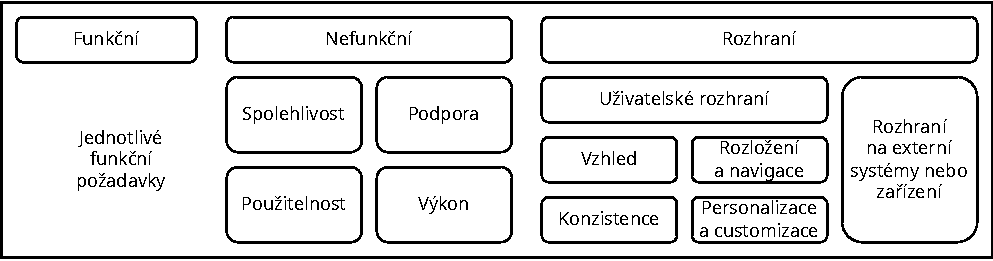
\includegraphics[width=0.95\textwidth]{img/pozadavky-diagram.pdf}
    \footnotesize \textit{Zdroj:} Vlastní zpracování
  \end{center}
\end{figure}

\FloatBarrier
\subsection{Funkční požadavky}\label{sekce:funkcni-pozadavky}

Funkční požadavky popisují konkrétní funkce, které musí systém poskytovat. Tedy určují, co by systém měl dělat \parencite{rejnkovaLokalizacePrizpusobeniMetodiky}. Funkční požadavky jsou formulovány v tabulce č. \ref{tab:funkcni-pozadavky} v samostatné příloze \ref{appendix:pozadavky} . Požadavky v tabulce mají unikátní identifikátor, název, podrobný popis, prioritu, která určuje důležitost požadavku (na škále důležitosti od 1 = vysoká,...,5 = nízká) a odkaz na případ užití, který tento požadavek ilustruje.

\subsection{Nefunkční požadavky}\label{sekce:nefunkcni-pozadavky}

Nefunkční požadavky jsou kvalitativními charakteristikami systému, které poskytují informace o omezeních a vlastnostech systému \parencite{rejnkovaLokalizacePrizpusobeniMetodiky}. Nefunkční požadavky byly dle šablony MMSP rozděleny na \textit{použitelnost}, \textit{spolehlivost}, \textit{výkon} a \textit{podporu}.

Požadavky na použitelnost aplikace jsou uvedeny v tabulce č. \ref{tab:POU-pozadavky}
Požadavky na spolehlivost systému byly stanoveny v tabulce č. \ref{tab:SPO-pozadavky}.
Požadavky na výkon systému byly stanoveny v tabulce č. \ref{tab:VYK-pozadavky}.
Požadavky na podporu se týkají aspektů vývoje a údržby systému \parencite{rejnkovaLokalizacePrizpusobeniMetodiky}. Tyto požadavky jsou popsány v tabulce \ref{tab:POD-pozadavky}.

\subsection{Požadavky na rozhraní}

Požadavky na rozhraní se dělí na požadavky na uživatelské rozhraní a na rozhraní na externí systémy nebo zařízení.

\subsubsection{Uživatelské rozhraní}

Požadavky na uživatelské rozhraní jsou zaměřeny na to, jak by mělo vypadat a fungovat uživatelské rozhraní systému \parencite{rejnkovaLokalizacePrizpusobeniMetodiky}. Tyto požadavky jsou rozděleny do čtyř kategorií, a to:
\textit{vzhled},
\textit{rozložení a navigace},
\textit{konzistence},
\textit{personalizace a customizace}.

Požadavky na vzhled mohou stanovit např. jaké barvy \parencite{rejnkovaLokalizacePrizpusobeniMetodiky} či jaký styl prvků budou použity. Vymezené požadavky na vzhled jsou uvedeny v tabulce č. \ref{tab:VZH-pozadavky}.

Požadavky na rozložení a navigaci jsou zaměřeny na to, jak by se uživatel měl v systému orientovat \parencite{rejnkovaLokalizacePrizpusobeniMetodiky}. Tyto požadavky jsou popsány v tabulce \ref{tab:ROZ-pozadavky}.

Požadavky na konzistenci se zaměřují na to, aby uživatelské rozhraní bylo jednotné a předvídatelné jako jiné systémy, které již uživatelé používají \parencite{rejnkovaLokalizacePrizpusobeniMetodiky}. Tyto požadavky jsou popsány v tabulce \ref{tab:KON-pozadavky}.

Požadavky na personalizaci a customizaci se týkají schopnosti systému přizpůsobit se individuálním potřebám, preferencím a charakteristikám uživatelů \parencite{rejnkovaLokalizacePrizpusobeniMetodiky}.
Požadavky lze vidět v tabulce \ref{tab:PER-pozadavky}.

\subsubsection{Rozhraní na externí systémy nebo zařízení}

Požadavky na rozhraní na externí systémy nebo zařízení se týkají schopnosti systému komunikovat a integrovat se s dalšími systémy, službami nebo zařízeními \parencite{rejnkovaLokalizacePrizpusobeniMetodiky}. Požadavky, které byly identifikovány jsou uvedeny v tabulce \ref{tab:EXT-pozadavky}.

\subsection{Systemová omezení}

Systémová omezení udávájí technická a jiná omezení, kterými je systém vázán \parencite{rejnkovaLokalizacePrizpusobeniMetodiky}. V případě této práce se jedná o požadavky uvedené v tabulce č. \ref{tab:SYS-pozadavky}.

\subsection{Požadavky na respektované standardy}

Tato sekce popisuje požadavky na respektované standardy, které musí systém dodržovat \parencite{rejnkovaLokalizacePrizpusobeniMetodiky}. Požadavky jsou uvedeny v tabulce č. \ref{tab:STA-pozadavky}. V případě této práce se jedná zejména o standardy vyplývající z OFN.

\subsection{Požadavky na dokumentaci}

Požadavky na dokumentaci říkají, co a jakým zposobem by mělo být dokumentováno a kdo za to odpovídá \parencite{rejnkovaLokalizacePrizpusobeniMetodiky}. V případě této práce se jedná o požadavky uvedené v tabulce č. \ref{tab:DOK-pozadavky}.


